
%(BEGIN_QUESTION)
% Copyright 2007, Tony R. Kuphaldt, released under the Creative Commons Attribution License (v 1.0)
% This means you may do almost anything with this work of mine, so long as you give me proper credit

Suppose you are asked to tune the controller of a liquid level process.  After obtaining permission from the operator, you analyze the response of the process variable (liquid level) to a 10\% up-and-down step change in the controller output (placed in manual mode):

$$\includegraphics[width=15.5cm]{i01727x01.eps}$$

The first thing you notice is that the PV trend is extremely noisy.  Investigating a little further, you find that the level transmitter is {\it ultrasonic}: it measures the height of liquid in the vessel by firing sound waves down at the liquid surface from above, and measuring the time delay of the echo.  Normally, ultrasonic level transmitters work well to measure liquid surface level, but in this process there are problems because the liquid's surface is constantly agitated by a powerful mixer inside the vessel which must be run constantly to prevent solids from settling and compacting at the bottom of the vessel.

How does the presence of this noise affect your decisions on how to tune it?  Would you tune this liquid level controller the same as you would any other liquid level controller, or would you tune it differently?  Explain your reasoning.

Furthermore, can you think of a way to obtain an accurate level measurement in this vessel without all the noise?

\vskip 20pt \vbox{\hrule \hbox{\strut \vrule{} {\bf Suggestions for Socratic discussion} \vrule} \hrule}

\begin{itemize}
\item{} Is it possible to tell from this trend whether the control valve {\it adds} liquid to the vessel or whether it {\it drains} liquid from the vessel?  Why or why not? 
\item{} Based on what you see here, does the controller need to be configured for {\it direct} action or for {\it reverse} action?
\item{} Suppose a fellow instrument technician recommended you activate the level transmitter's {\it damping} function in order to help stabilize the PV trend.  Would you agree with this line of action?  Explain why or why not.
\end{itemize}

\underbar{file i01727}
%(END_QUESTION)





%(BEGIN_ANSWER)

This is definitely an {\it integrating} process, and as such it would normally respond well to aggressive proportional action.  However, with all the noise present, proportional action will cause the control valve to ``jump'' noisily as well, prematurely wearing out its packing and consuming a lot of instrument air in the process!

Probably the best way to minimize noise in the process measurement is to equip the ultrasonic level transmitter with a {\it stilling well}.

%(END_ANSWER)





%(BEGIN_NOTES)

The integrating nature of this process is revealed by two traits: the roughly constant slope (linear shape) of the process response following the output step-change, and also the fact that the process variable levels off and stabilizes at a new value when the output returns to its former value.

In a case like this, I would suggest not tuning the controller at all until the process noise problem was eliminated.  Until the noise is significantly mitigated, we cannot implement the aggressive proportional action this process needs so much.






\vfil \eject

\noindent
{\bf Summary Quiz:}

Explain why {\it derivative} (rate) control is to be avoided in the loop controller when the process variable is ``noisy.''

\begin{itemize}
\item{} Derivative will cause a ``noisy'' PV to grossly overshoot the SP every time
\vskip 5pt 
\item{} The use of derivative action causes an error to develop between PV and SP
\vskip 5pt 
\item{} Derivative action will cause the control valve to exhibit hysteresis
\vskip 5pt 
\item{} Proportional-only control is sufficient by itself to regulate any ``noisy'' process
\vskip 5pt 
\item{} ``Noise'' will be interpreted by the controller as very high rates of change
\vskip 5pt 
\item{} The controller will not allow you to apply damping if derivative action is used
\end{itemize}

%INDEX% Control, PID tuning: predicting PID requirements based on open-loop response

%(END_NOTES)


